%\documentclass{article}
%\usepackage[demo]{graphicx}
%\usepackage{subfig}
%\usepackage{tikz}
%\usepackage{multirow}
%\usepackage{siunitx}
%\begin{document}
%\begin{figure}
%%%%%%%%%%%%%%%%%%%%%%%%%%%%%
%\begin{tabular}{cc}
%Fig A & \multirow{3}{*}{Fig D}\\
%Fig B & \\
%Fig C & \\
%\end{tabular}
\noindent\makebox[\textwidth]{%
\begin{tabular}{cc}
%%%%% LEFT TOP %%%%%
	\subfloat[\SI{180}{\degree-scan}]{
		%%%%%
		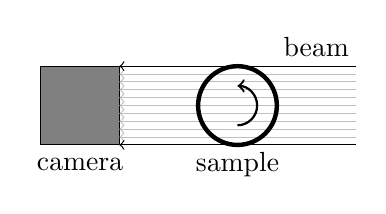
\begin{tikzpicture}
			%drawing grid
			%\draw[color=gray] (0,0) grid (8,1);
			\def\start{0}
			\def\length{1}
			%camera
			\draw [fill=gray] (\start,\start) rectangle (\length,\length);
			\node at (.5*\length,-.25) {camera};
			% beam
			\foreach \x in {0,.1,...,1.1}
				\draw[gray!50,<-] (\length,\x) -- (4*\length,\x);
			\foreach \x in {0,\length}
				\draw[<-] (\length,\x) -- (4*\length,\x);
			\node at (3.5*\length,\length+.25) {beam};
			%sample
			\draw[ultra thick] (2.5*\length,0.5*\length) circle (.5*\length);
			\draw[thick,->] (2.5*\length,0.25*\length) arc (-90:90:.25*\length);
			\node at (2.5*\length,-.25) {sample};
		\end{tikzpicture}
		%%%%%
		\label{subfig:180degreescan}
	}%
& %%%%% RIGHT TOP %%%%%
	\multirow{3}{*}{%
	\subfloat[Stacked scanning for long and thin samples]{
		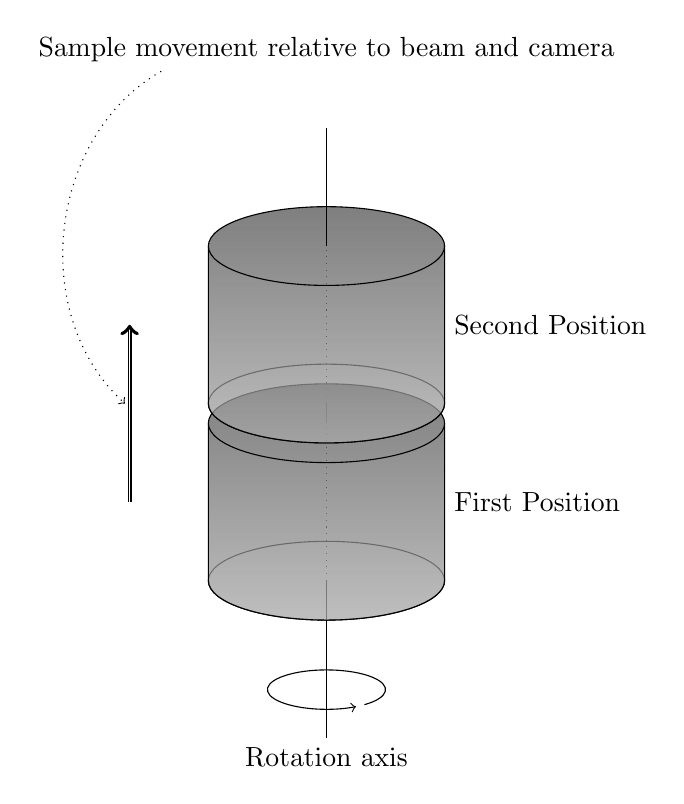
\begin{tikzpicture}%[ultra thick,scale=1]%,show background grid]
			%draw axes
				%\draw[ultra thick] (-10,0) -- (10,0);
				%\draw[ultra thick] (0,-10) -- (0,10);
				%\draw[ultra thick] (0,0) circle (.125);
			% rotation axis
				\draw[->] (0,-2) ++ (-50:.75) arc (-50:300:.75 and .25);
				\draw (0,-3) node [below] {Rotation axis} -- ++(0,2);
				\draw[dotted] (0,-1) -- ++(0,2);
				\draw (0,1) -- ++(0,0.25);
				\draw[dotted] (0,1.25) -- ++(0,2);
			% position 1
				\draw (0,-1) circle (1.5 and .5);
				\fill[shade,semitransparent] (-1.5,-1) arc (-180:0:1.5 and .5) -- ++(0,2) arc (0:180:1.5 and .5) -- cycle;
				\draw (-1.5,-1) arc (-180:0:1.5 and .5) -- ++(0,2) arc (0:180:1.5 and .5) -- cycle;		
				\draw (-1.5,1) arc (-180:0:1.5 and .5);
				\draw (1.5,0) node [right] {First Position};
			% position 2
				\draw (0,1.25) circle (1.5 and .5);
				\fill[shade,semitransparent] (-1.5,1.25) arc (-180:0:1.5 and .5) -- ++(0,2) arc (0:180:1.5 and .5) -- cycle;
				\draw (-1.5,1.25) arc (-180:0:1.5 and .5) -- ++(0,2) arc (0:180:1.5 and .5) -- cycle;		
				\draw (-1.5,3.25) arc (-180:0:1.5 and .5);
				\draw (1.5,2.25) node [right] {Second Position};
			% rotation axis on top
				\draw (0,3.25) -- ++(0,1.5);									
			% sample movement
				\draw[double,->] (-2.5,0) -- (-2.5,2.25) ;% node [text width=10cm,midway,left] {Sample movement relative to beam and camera};	
				% sample movement
				\node (movefrom) at (0,5.75) {Sample movement relative to beam and camera};
				\node (moveto) at (-2.5,1.125) {};
				\draw [->,dotted] (movefrom) to [bend right=54] (moveto);
		\end{tikzpicture}
		\label{subfig:stackedscan}
	}%
	}
\\
%%%%% LEFT MIDDLE %%%%%	
	\subfloat[\SI{360}{\degree-scan}]{
		%%%%%
		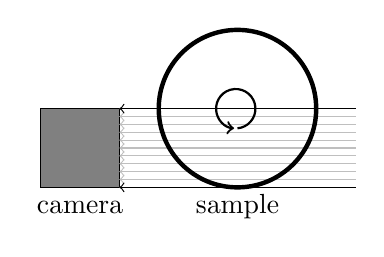
\begin{tikzpicture}
			%drawing grid
			%\draw[color=gray] (0,0) grid (8,1);
			\def\start{0}
			\def\length{1}
			%camera
			\draw [fill=gray] (\start,\start) rectangle (\length,\length);
			\node at (.5*\length,-.25) {camera};
			% beam
			\foreach \x in {0,.1,...,1.1}
				\draw[gray!50,<-] (\length,\x) -- (4*\length,\x);
			\foreach \x in {0,\length}
				\draw[<-] (\length,\x) -- (4*\length,\x);
		%	\node at (3.5*\length,\length+.25) {beam};
			%sample
			\draw[ultra thick] (2.5*\length,\length) circle (\length);
			\draw[thick,->] (2.5*\length,\length-0.25*\length) arc (-85:265:0.25*\length);
			\node at (2.5*\length,-.25) {sample};
		\end{tikzpicture}
		%%%%%
		\label{subfig:360degreescan}
	}%
& %%%%% RIGHT MIDDLE %%%%%
\\
%%%%% LEFT BOTTOMT %%%%%
	\subfloat[wide field scan]{
		%%%%%
		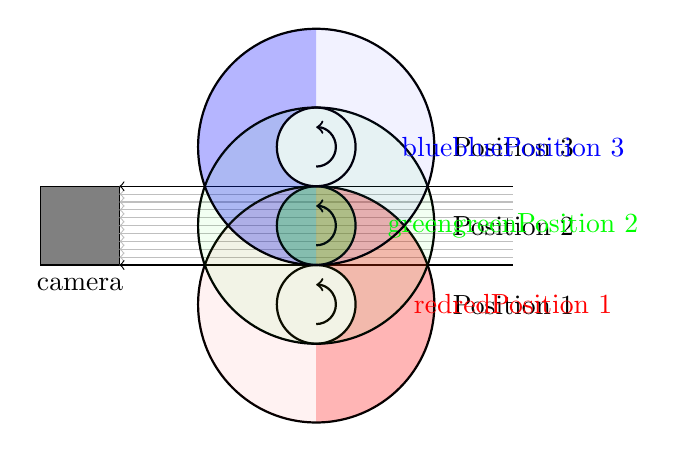
\begin{tikzpicture}
			\def\length{1}
			\def\beamlength{6}
			%grid
		%	\draw[color=gray] (0,-3) grid (7,3);
			%camera
			\draw [fill=gray] (0,0) rectangle (\length,\length);
			\node at (.5*\length,-.25) {camera};
			% beam
			\foreach \x in {0,.1,...,1.1}
				\draw[gray!50,<-] (\length,\x) -- (\beamlength,\x);
			\foreach \x in {0,\length}
				\draw[<-] (\length,\x) -- (\beamlength,\x);
		%	\node at (3.5*\length,\length+.25) {beam};
		%%%%%	%colored samples
		%%%%%	\foreach \y/\color/\position in {-.5/red/1,.5/green/2,1.5/blue/3}
		%%%%%		{
		%%%%%			\draw[thick,color=\color] (0.5*\beamlength+0.5*\length,\y) circle (1.5*\length) circle (.5*\length);
		%%%%%			\draw[thick,->,color=\color] (0.5*\beamlength+0.5*\length,\y-.25*\length) arc (-90:90:0.25*\length);
		%%%%%			\node[color=\color] at (\beamlength,\y) {Position \position};
		%%%%%		}
			% filled samples
			\fill [color=red,nearly transparent]   (3.5,1) arc (90:-90:1.5*\length) -- ++(0,1) arc (-90:90:.5*\length);
			\fill [color=blue,nearly transparent]  (3.5,3) arc (90:270:1.5*\length) -- ++(0,1) arc (270:90:.5*\length);
			\fill [color=green,nearly transparent] (0.5*\beamlength+0.5*\length,.5) circle (0.5*\length);	
			\foreach \y/\position/\color in {-.5/1/red,.5/2/green,1.5/3/blue}
				{
					\draw[thick] (0.5*\beamlength+0.5*\length,\y) circle (1.5*\length) circle (.5*\length);
					\draw[thick,->] (0.5*\beamlength+0.5*\length,\y-.25*\length) arc (-90:90:0.25*\length);
					\fill [color=\color,ultra nearly transparent] (0.5*\beamlength+0.5*\length,\y) circle (1.5*\length);
					\node at (\beamlength+.005,\y-.005) {Position \position};
					\node [color=\color] at (\beamlength,\y) {Position \position};
				}
		\end{tikzpicture}
		%%%%%
		\label{subfig:widefieldscan}
	}%
& %%%%% RIGHT BOTTOM %%%%%
\\
\end{tabular}
} %makebox
%%%%%%%%%%%%%%%%%%%%%%%%%%%%%	
%\caption{Caption of subfigures \subref{subfig:180degreescan}, \subref{subfig:360degreescan}, \subref{subfig:widefieldscan} and \subref{subfig:stackedscan}}
%\end{figure}
%\end{document}